\documentclass[a4paper,12pt]{article}

\usepackage[T1]{fontenc}
\usepackage[utf8]{inputenc}
\usepackage[english, polish]{babel}
\usepackage{lmodern}
\usepackage{graphicx}
\usepackage{fancyhdr}
\usepackage{float}
\usepackage{array}
\usepackage{hyperref}
%\usepackage{mathtools}


\setlength{\textheight}{23.5cm}
\setlength{\textwidth}{15.92cm}
\setlength{\footskip}{10mm}
\setlength{\oddsidemargin}{0mm}
\setlength{\evensidemargin}{0mm}
\setlength{\topmargin}{0mm}
\setlength{\headsep}{15mm}
\setlength{\parindent}{0cm}
\setlength{\parskip}{2.5mm}
%nowa extra row do tabeli :)  :) 
\setlength{\extrarowheight}{4pt}

\author{Justyna Ilczuk, Jacek Rosiński}

\begin{document}

\begin{center}

    \begin{tabular}{ | m{5cm}| m{5cm} | m{5cm} |}
    \hline 
    \multicolumn{2}{|c|}{{ \Large \textbf{Laboratorium Fizyki 2}} }
    &  
    \begin{center}
    Data wykonania ćwiczenia:
    \end{center}
    \begin{center}
      16.10.2013 
    \end{center}
    \begin{center}
    Środa 9.45-13.45
    \end{center}
     \\ 
    
    \hline
    \multicolumn{2}{|c|}{Justyna Ilczuk \newline Jacek Rosiński}
    & \begin{center}
    {\small Data złożenia sprawozdania:} \newline \today
    \end{center}   \\
   	
   	\hline
    Wydział Fizyki & Grupa: K-1 \newline Rok akademicki: 2013/2014 &  \\
   	\hline
   	\multicolumn{2}{|l|}{Prowadzący: Michał Marzanotowicz} & \multicolumn{1}{|l|}{Ocena końcowa:}\\
    \hline
    \end{tabular}
\end{center}

\newpage

\pagestyle{fancy}
\fancyfoot[CO]{\ }
\fancyhead[RO]{\footnotesize{\thepage} }
%\fancyhead[RO]{\footnotesize{\ } }
\fancyhead[LO]{Justyna Ilczuk i Jacek Rosiński K-1, Diody fotowoltaiczne }

% wrzucanie wykresów:

%\begin{figure} [H]
%  \begin{center}
%    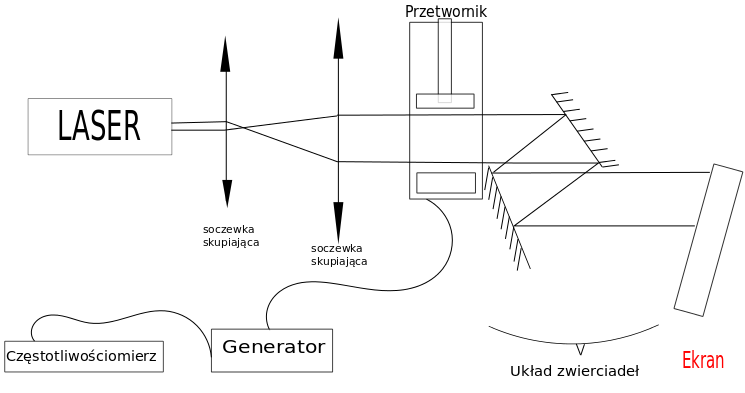
\includegraphics[width = 15cm]{Rysunek.png}
%    \caption{Układ pomiarowy}
%  \end{center}
%\end{figure}


\section{Cel ćwiczenia}
Pomierzyć sobie próbki i zobaczyć i zrozumieć co tam się fajnego w środku dzieje.

\section{Wyniki pomiarów}

Dla jednej próbki mierzyliśmy charakterystyki jasne i ciemne.
Dla drugiej próbki mierzyliśmy tylko charakterystyki jasne.

A dla trzeciej próbki liczylismy koncentrację nośników (dziur chyba?).

Poniżej przedstawiamy wykresy charakterystyk diod w zależnosci od temperatury dla dwóch badanych próbek.

\begin{figure} [H]
  \begin{center}
    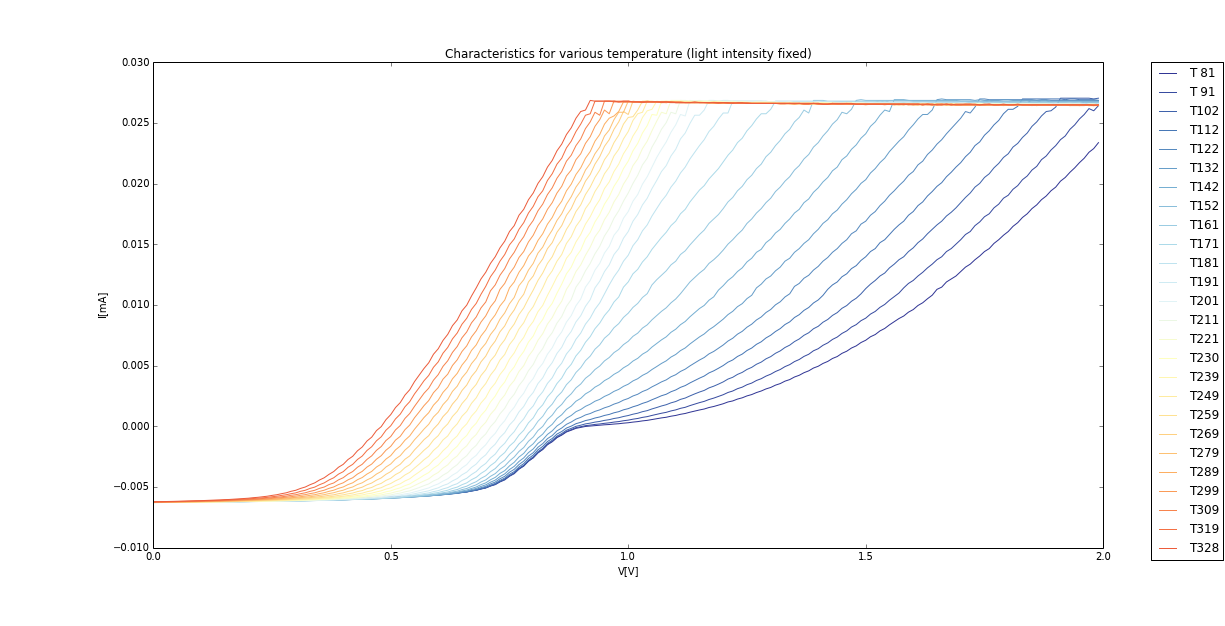
\includegraphics[width = 15cm]{probka1_temperatura.png}
    \caption{Próbka 1 - charakterystyki dla różnych temperatur}
  \end{center}
\end{figure}

\begin{figure} [H]
  \begin{center}
    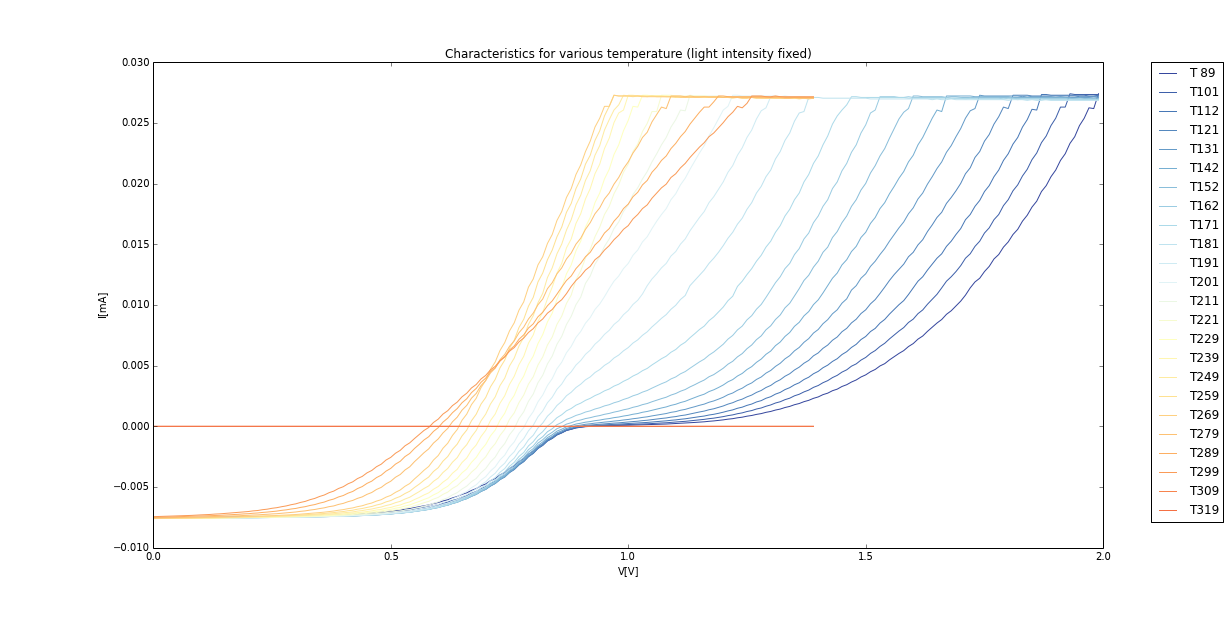
\includegraphics[width = 15cm]{probka2_temperatura.png}
    \caption{Próbka 1 - charakterystyki dla różnych temperatur}
  \end{center}
\end{figure}

Dalej przedstawiamy wykresy dla różnych wartości natężeń światła.
\begin{figure} [H]
  \begin{center}
    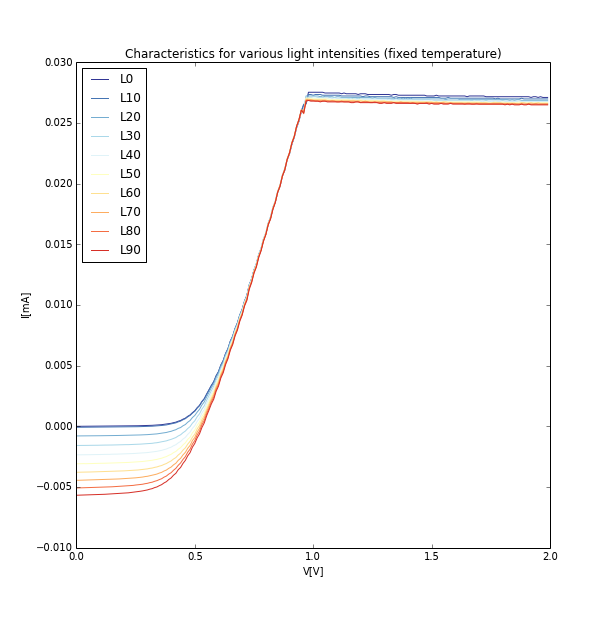
\includegraphics[width = 15cm]{probka1_swiatlo.png}
    \caption{Próbka 1 - charakterystyki dla różnych natężeń światła}
  \end{center}
\end{figure}

\begin{figure} [H]
  \begin{center}
    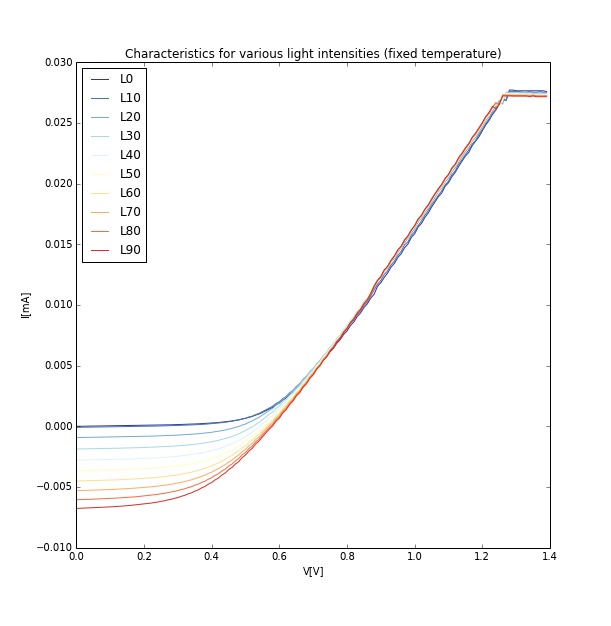
\includegraphics[width = 15cm]{probka2_swiatlo.png}
    \caption{Próbka 1 - charakterystyki dla różnych natężeń światła}
  \end{center}
\end{figure}

\begin{figure} [H]
  \begin{center}
    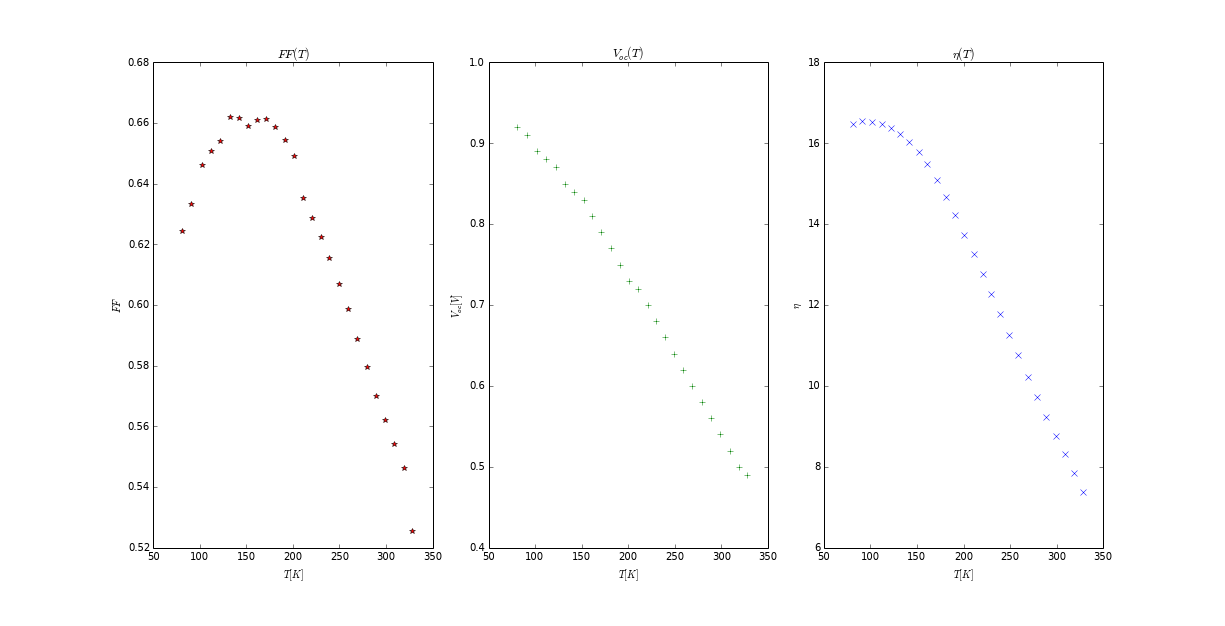
\includegraphics[width = 15cm]{probka1_rozne.png}
    \caption{Fantastyczny wykres}
  \end{center}
\end{figure}

\begin{figure} [H]
  \begin{center}
    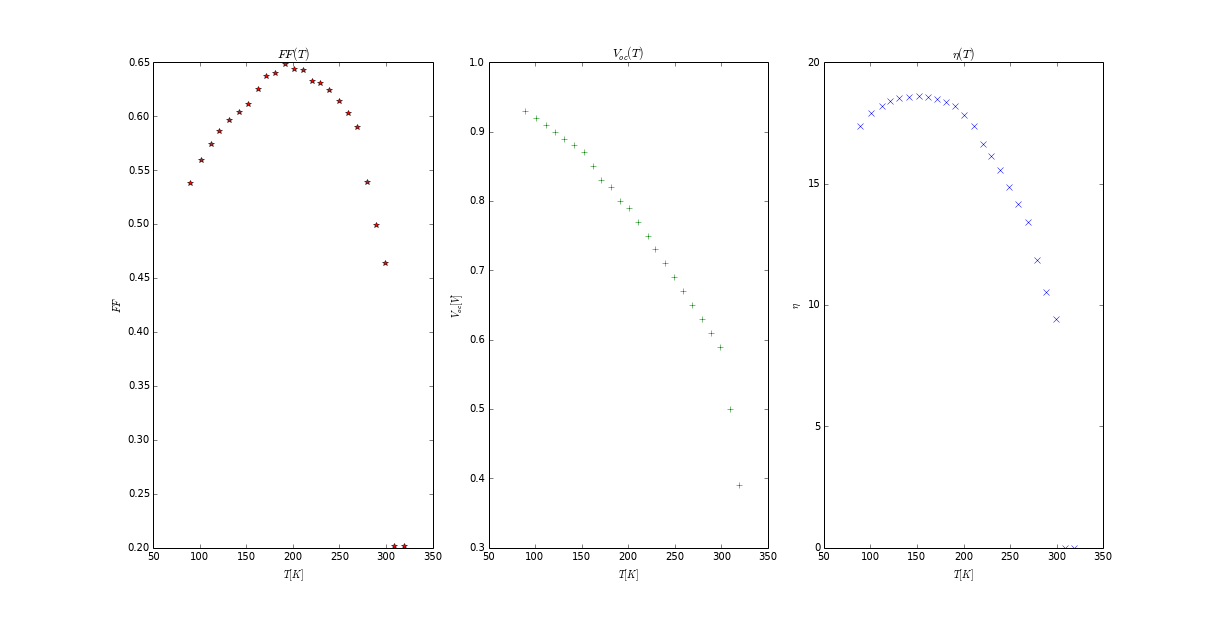
\includegraphics[width = 15cm]{probka2_rozne.png}
    \caption{Fantastyczny wykres}
  \end{center}
\end{figure}


\begin{figure} [H]
  \begin{center}
    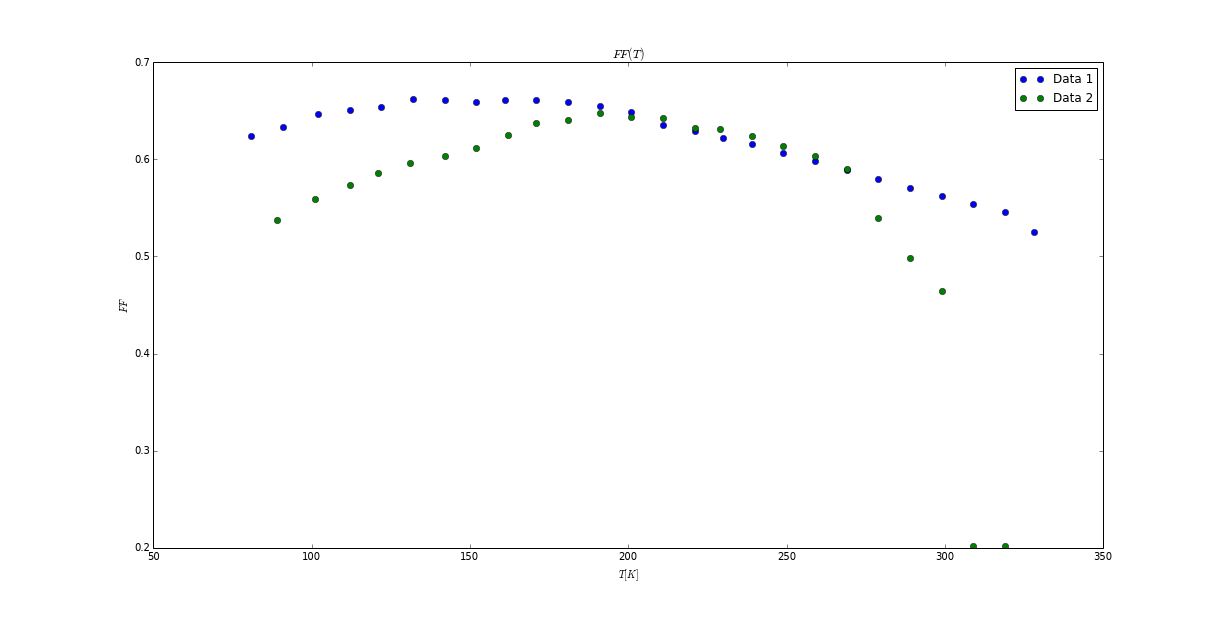
\includegraphics[width = 15cm]{probki_porownanie_FF.png}
    \caption{Fantastyczny wykres}
  \end{center}
\end{figure}

\begin{figure} [H]
  \begin{center}
    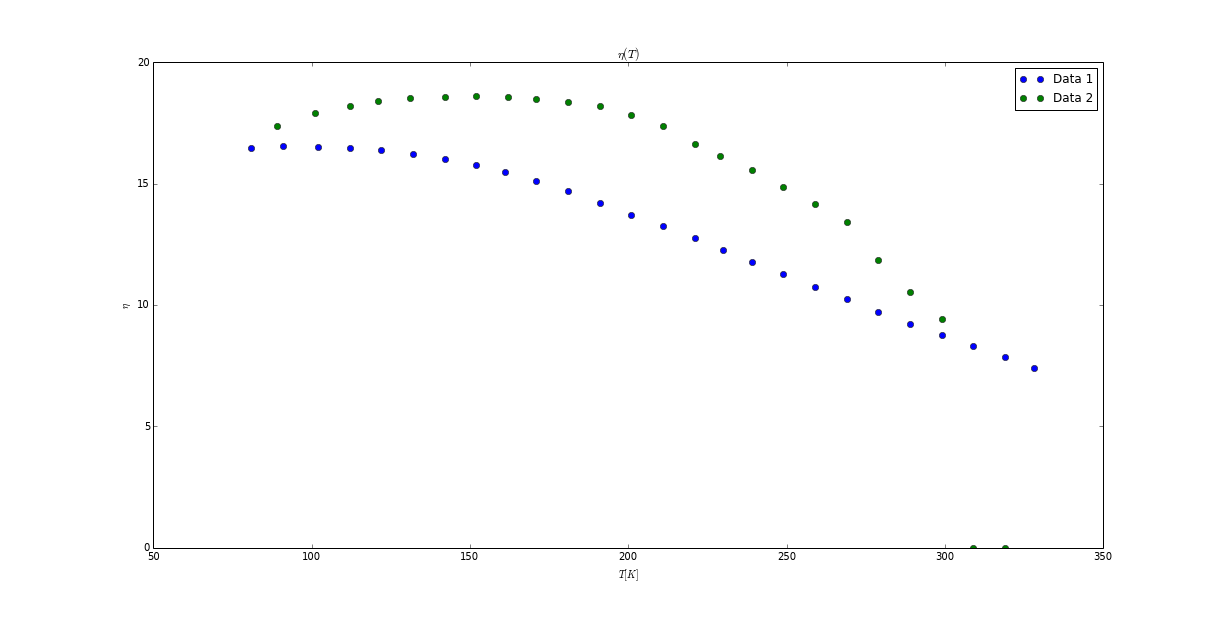
\includegraphics[width = 15cm]{probki_porownanie_eta.png}
    \caption{Fantastyczny wykres}
  \end{center}
\end{figure}

\begin{figure} [H]
  \begin{center}
    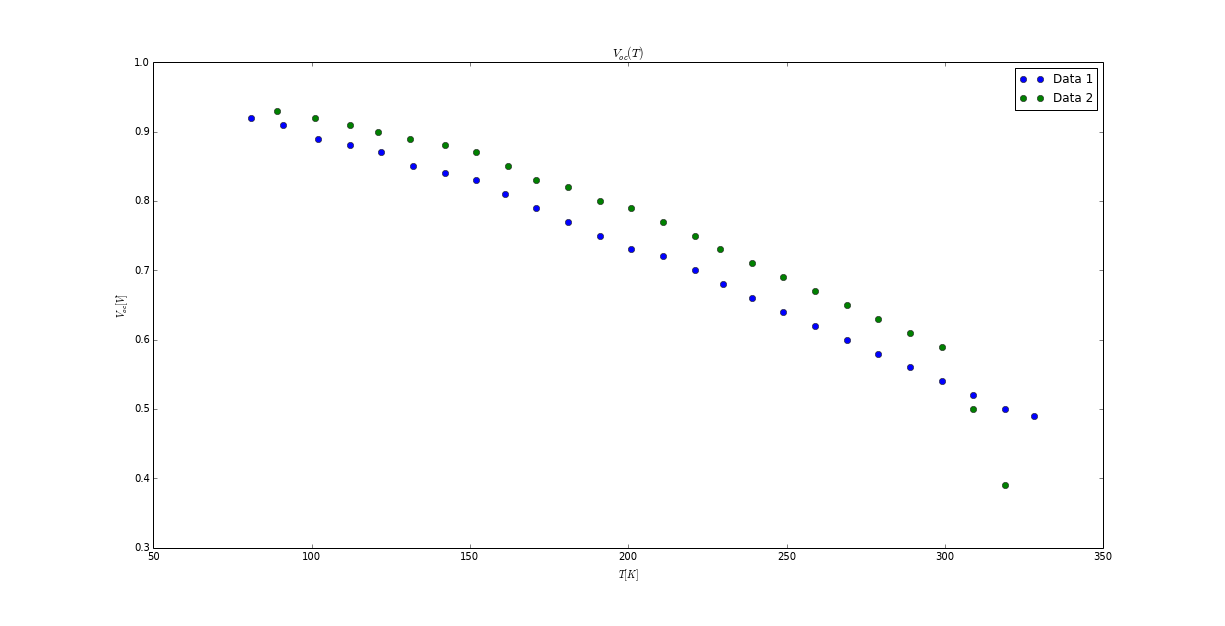
\includegraphics[width = 15cm]{probki_porownanie_V_oc.png}
    \caption{Fantastyczny wykres}
  \end{center}
\end{figure}

\begin{figure} [H]
  \begin{center}
    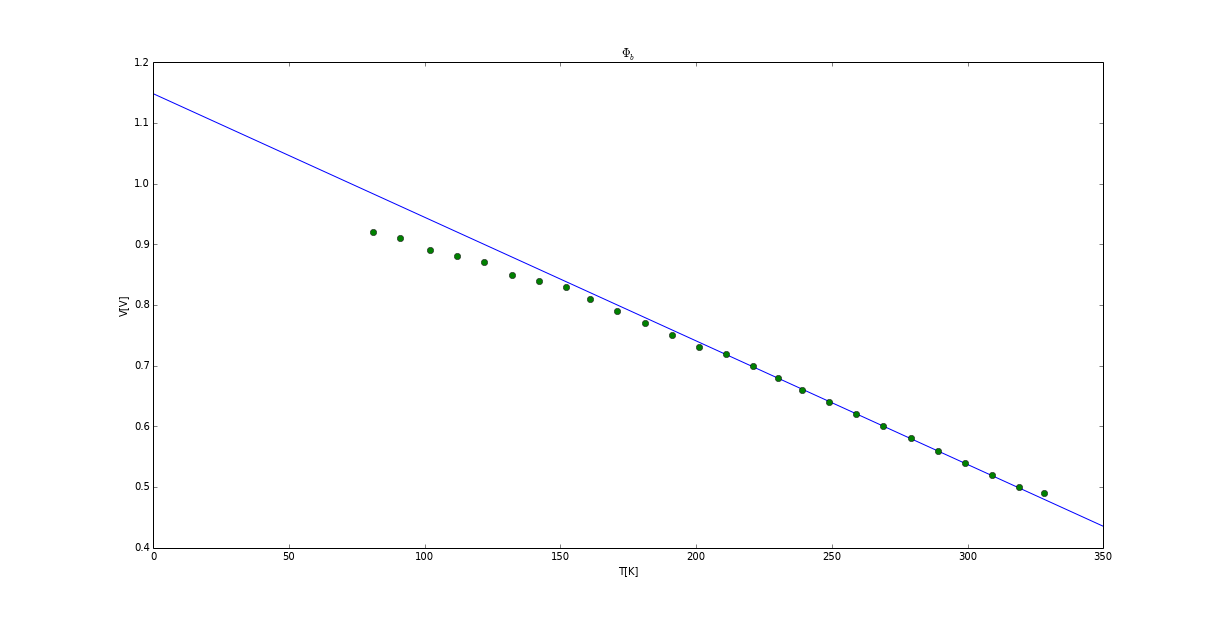
\includegraphics[width = 15cm]{probka1_phi_b.png}
    \caption{Fantastyczny wykres}
  \end{center}
\end{figure}

\begin{figure} [H]
  \begin{center}
    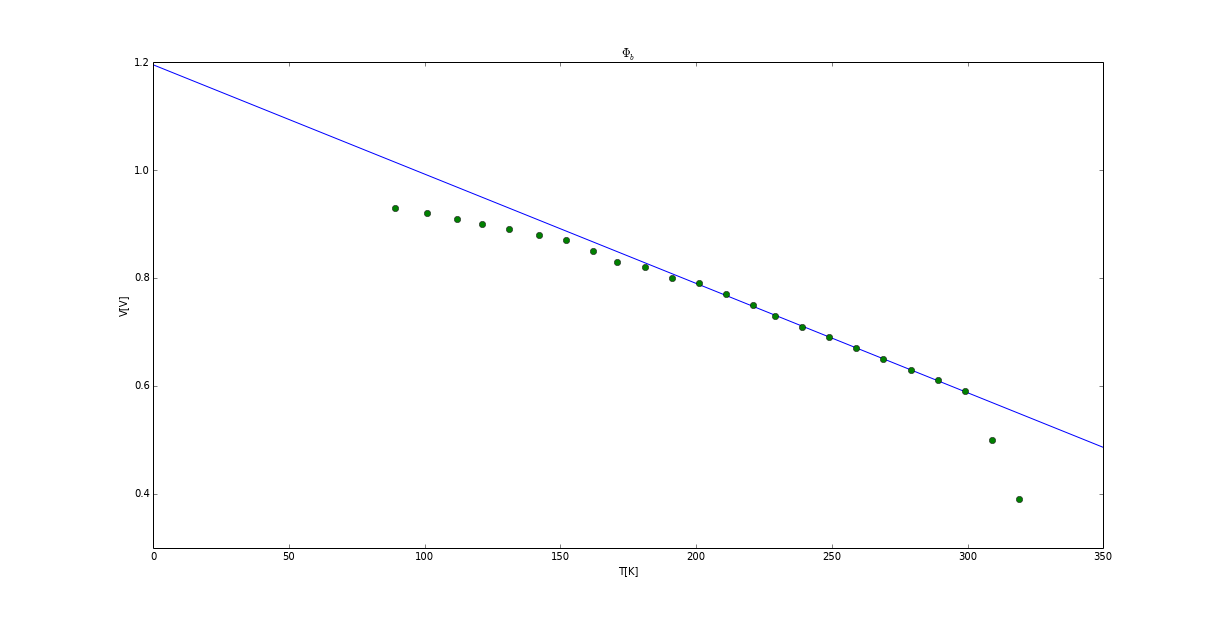
\includegraphics[width = 15cm]{probka2_phi_b.png}
    \caption{Fantastyczny wykres}
  \end{center}
\end{figure}


\begin{figure} [H]
  \begin{center}
    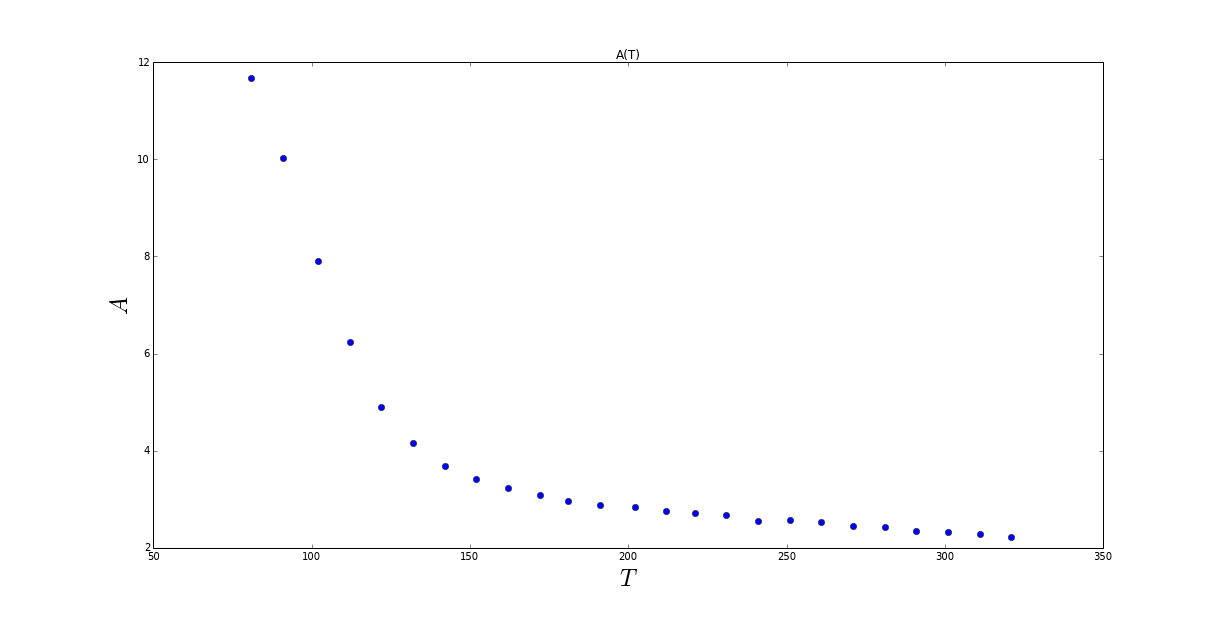
\includegraphics[width = 15cm]{A_T.png}
    \caption{Fantastyczny wykres}
  \end{center}
\end{figure}

\begin{figure} [H]
  \begin{center}
    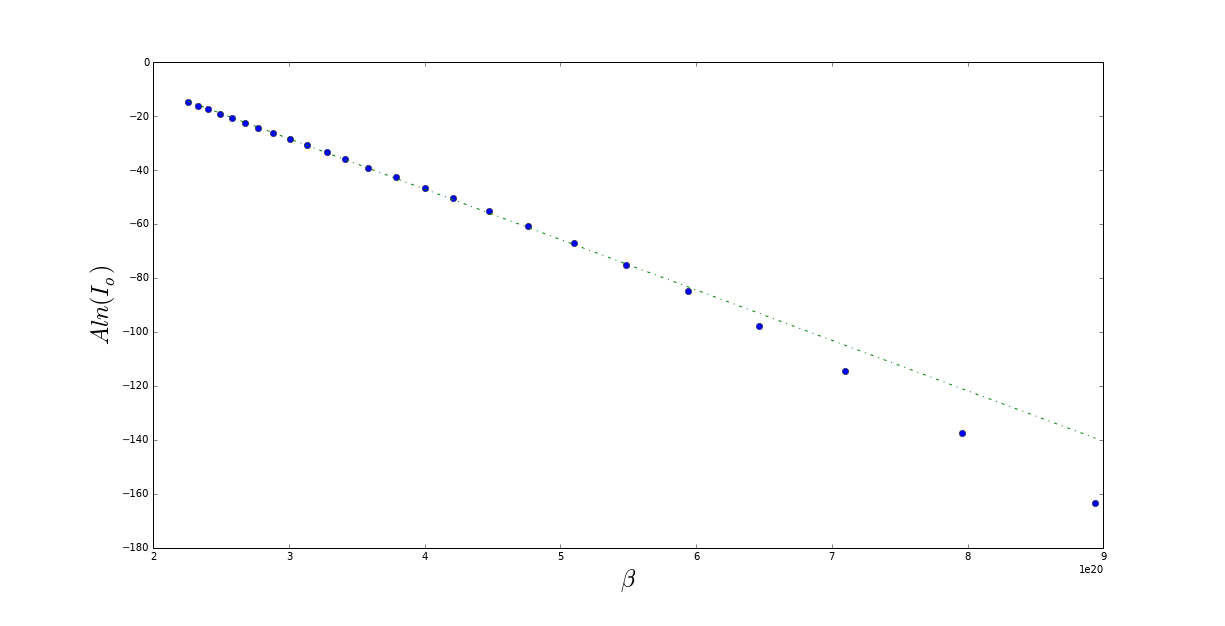
\includegraphics[width = 15cm]{A_lnI.png}
    \caption{Fantastyczny wykres}
  \end{center}
\end{figure}
\section{Wstęp}

\section{Wnioski}

\end{document}
